

% Laatu painottuu startupissa siihen, mitä asiakkaat ja loppukäyttäjät pitävät tärkeänä
% Laadun merkitys elinkaaren eri vaiheissa muuttuu
%	-Aluksi tärkeintä validoida featuret ja idea
%	-Laadussa tärkeää aluksi hyvä muokattavuus, refaktoroinnit, asiakkaalle kriittisten osien testaus
%	-Elinkaaren alussa ei väliä matalan prioriteetin bugeilla tai featureiden vajaalla toiminnalla
%	-Kun idea alkaa olla validoitu, muuttuu laadun merkitys tuotteistuksen yhteydessä
%	-Laatuun on käytössä myöhemmin enemmän resursseja, koska asiakkaita alkaa olla
%	-Osuiskohan tähän Lean Startupin skaalausvaihe

 \section{Quality in a Startup project}

In the beginning of the chapter about role of quality, Eric Ries states that "The best professionals and craftpersons alike aspire to build quality products; it is a point of pride". This is a good summary about the attitude towards software quality in many movements about modern software development. Measuring and defining quality in modern software projects with constant changes and uncertainty can be difficult, but the development personnel should have the pursuit for high quality.

Ries claims that modern production processes seek to boost efficiency by relying to high quality. The belief that the customer is the most important part of the production process means that all effort should be focused to producing results that the customer finds valuable. This view can be beneficial in an environment where the company knows the opinions of customers. However, in a startup development, assuming the opinions of customers is a risky thing to do. Often in the startup, it is not even sure who the customer is. Thus, Ries introduces a quality principle for startups: "If we do not know who the customer is, we do not know what quality is".

In a startup developing an MVP, the quality of the product can be a fluid concept. Even if the quality of MVP is low for customers, it can bring great value in building a high-quality product. If the customers find the product low on quality, this can be used as an opportunity to learn what customers care about. This is infinitely better than mere speculation, because it provides empirical information on which to build future products.

When working with a 3D chat software called IMVU, Ries and his colleagues decided to leave a critical sophisticated feature done with only minimum effort. They were embarrassed to release the moving of the avatars without any animations or other modern visualizations. The avatars just reappeared to another location. The response of the customers was surprising as the customers were thrilled from the new feature, which allowed an immediate change of location without waiting. From the customers point of view, the released feature was more appropriate than the option which would take more time and money to implement. In the end, the quality of the released feature was probably higher than the one planned. The lesson behind the story is that customers do not care how much time something takes to build.

Lean Startup method is aiming for the goal of winning over customers and not opposed to building high-quality products. Thus, it is necessary to set aside some professional standards to enable the validated learning as soon as possible. This is not supposed to allow operating in an undisciplined manner. This is important as there are some quality problems that can slow down the Build-Measure-Learn feedback loop. In addition, defects complicate the evolution of the product and interfere with the ability to learn. Helping the development of the MVP means removing any feature, process or effort that does not lead directly to the learning sought.~\cite{ries2011lean}

\section{Foundations of high quality}

TODO: Johdatus

 \subsection{Clean code} 

 Every programmer with experience for more than two or three years have probably been slowed down by messy code. Over a couple of years of development, teams that were moving fast at the beginning of the project can be slowed down to a really slow pace. Development begins to include more and more non-trivial changes, which are about resolving the existing knots and tangles and adding new. Eventually, the mess can become so big that it can not be cleaned up at all. The total cost of owning a mess is being pondered by Robert C. Martin in his book Clean Code: A Handbook of Agile Software Craftmanship.

 Martin reminds that "code is really the language in which we ultimately express the requirements" and thus code is in the very foundations of every software project. A common mistake done in software projects is to increase the measure of developers in the team. This is usually done when the code has already reached a too messy state and the pace of development has slowed down. Adding new staff to the development does not improve the situation, but underlines the meaning of messy code. This new staff is not familiar with the existing system, so they easily complicate the system even further, driving the productivity even worse.

 A bitter fact for the developers is that usually the cause of messy code is the fault of the developers. While the management and sales staff are defending schedules and requirements, the developers should be defending the code. Many developers previously slowed down by messy code still feel the pressure of deadlines and the temptation to make messes to achieve them. Martin says that true professionals know that the only way to go fast is to keep the code as clean as possible at all times. A programmer able to write clean code is an artist, who can use all the little techniques in a disciplined manner through the sense of cleanliness.~\cite{martin2008clean}
 
 \subsection{Integrity} 

 One of the principles of Lean Software Development (LSD) is "Build Integrity In", which has its premises in high-performing automotive companies in 1980s. A study "Product Development Performance" by Kim Clark found out that the product integrity was a key difference between average and high-performing companies in developing superior products. Clark found out that integrity has two dimensions: external integrity and internal integrity.~\cite{clark1991product}

 LSD renames these two types of integrities as perceived integrity and conceptual integrity. Perceived integrity is a balance of function, usability, reliability and economy observed by the customer. It is affected by the whole experience of the system beginning from advertising and delivery to intuitiveness and the ability to solve the problem. An analogy to the measure of perceived integrity comes from the question: which ones of the bookmarks of your browser would you add back immediately, if you wiped out them all? These are the products with perceived integrity. 

 Conceptual integrity is smoothness and uniformity of the whole system's central concepts. The architecture of the system has an effective balance between flexibility, maintainability, efficiency and responsiveness. Conceptual integrity is a prerequisite to perceived integrity. To be able to achieve perceived integrity, the system must have a consistent design. As the system evolves and matures, conceptual integrity emerges. Although conceptual integrity is needed for perceived integrity, the existence of the former does not ensure the existence of the latter. This is because conceptual integrity is not sufficient for a successful customer experience, if the system does not meet the users' need.~\cite{poppendieck2003LSD}

\section{Aiming towards high quality}

JOHDATUS

\subsection{Build Integrity In} 

In the study by Kim Clark, a primary claim is that integrity is achieved through superior information flow. Perceived integrity is a projection of the integrity of the information flow between users and developers. In turn, conceptual integrity is a projection of the integrity of the upstream and downstream of technical information flow. When reaching a system with high perceived and conceptual integrity, an excellent information flow is necessary both between customer and development team and between the upstream and downstream processes of the development team. Information flows must take into account both the current and potential uses of the system.

\textbf{Perceived integrity.} In traditional software development, perceived integrity is transmitted to programmers through a multistage process. In this process, requirements are collected and processed through analysis and design. Then the design is transfered to the programmers implementing the code. These multiple hand-offs will cause the loss of considerable amount of information, key details and future perspectives. Fortunately, an alternative for this multistage process is to establish a superior customer-developer information flow by other means. With smaller systems, the development should be done by a single team having direct access to the people capable of judging the systems integrity. This team should use short iterations in where the system is demonstrated to a wide range of people giving feedback about the integrity. This way the feedback can be used for a rapid steering of course. Another technique is to use customer tests purposely created for getting feedback.

% Communicating two-ways face to face in small batches and solving the problems at the same time
\textbf{Conceptual integrity.}
Conceptual integrity in automotive manufacturing is pursued by using existing parts and integrated problem solving. In integrated problem solving, understanding and solving the problem happen simultaneously, instead of sequentially. The initial information is released early and not only after complete information is available. Information flow happens in two directions instead of one and it contains multiple small batches of information instead of a single large batch. The preferred communication style is face to face instead of documents. This kind of problem-solving is ideal for achieving conceptual product integrity, particularly in development of complex systems such as automobiles or software systems.

In software development, using integrated problem solving means that the development must be started before the design is finalized. In addition, the developers should be able to access customers or customer representatives for getting the answers as soon as possible for any questions raised. Customer tests should be developed and ran along the iterations and not just at the end.

Finally, using experienced developers in their own areas of expertise can help in achieving conceptual integrity. Not all of the developers have to be with plenty of experience, but for the complex areas, experience brings understanding of the technical details and patterns widely used to manage with the complexities. One of these experienced developers should be a master developer facilitating the effort over multiple teams. For example, integrating the decisions and trade-offs among multiple developers and customers would be the responsibility of the master developer.

\textbf{Refactoring.} When the integrity of a product is building, the iterative development brings continuous improvement as the product is evolving. In software development, the system must be continuously improved by the developers. Otherwise the internal structures of the software will become calcified and fragile. In time, the system will even stop working. Refactoring is done to prevent this disintegration of the software structures over the development.

The need for refactoring comes when new features are added to the system one at a time and the architecture and requirements of the system change gradually. Often it would be better to think of new related features as a set and build an architectural capability to support them. If the features are added in multiple different locations of the code, the system will lose conceptual integrity. Refactoring regularly keeps the system healthy.

TODO: p. 142-144

\textbf{Testing.} In a traditional software development where implementation is done single module at a time, there are numerous types of testing used. There are for example unit testing, system testing, integration testing and acceptance testing used. The purpose of testing is to check that the intention behind the design is achieved and the system does what the customers want it to. In LSD, the development is done by implementing entire features instead of single modules, so the distinction between the different kinds of testing is more artificial. Instead, testing is divided into two parts: developer tests and customer tests. Developer tests are testing that the implemented features work as intended and that all the pieces work together. Customer tests are developed to verify that the system does what customers expect.

Tests act in several different roles in the development process. First, they present the exact functioning that the features are supposed to have. Second, they also supply information on whether the features actually work as supposed. Third, tests act as a scaffolding which provides support for tools such as refactoring. This allows the developers to make changes during the development. Fourth, after the development is done, the tests provide a representation of how the system was built. Finally, developing sufficient tests for all systems in production, making changes to these systems can be verified by running the tests for all related applications.

Tests can also work as a tool for communication. Customer tests can be written within the conversation with the customer about details of desired functionality. This way the tests can give the most accurate description of how the features should work for a customer. Likewise, developers can document the planned design by writing tests testing exactly what the design should do. There are other tools allowing the communication before the code is written, but there is no substitute for testing whether the system does what it is supposed to do. With this in mind, using tests for both tasks can be beneficial.

Receiving immediate feedback about the correct operation of code is important to a developer. The developer usually somehow tests the code as soon as its written, so the test could be captured as a written test allowing the reuse. Another opportunity to catch necessary experiments as tests is the review to customer within an iteration. Demonstrating the current system to a customer can be done with a set of demos or scripts, which can be captured as customer tests. These captured tests should be run as often as possible, so the team should ensure that the tests will not take too much time and are automated as much as possible.

Using automated testing with extensive test suites for both developer testing and customer testing can be an efficient way to implement scaffolding to support the development. The scaffolding is a structure supporting the developers when they are making major changes to the system. While developing software in iterations, refactoring and other tools will include changes, which tend to have unintended effects. Having these effects in the system without the scaffolding provided by automatic tests can be an unsustainable situation. Often it may seem that writing tests slows down the development, but it pays back both during development and over the systems life cycle.

\subsection{Empower the Team}

Lean thinking emphasized the importance of intelligent, disciplined and motivated frontline workers. In LSD, it is believed that the critical factor in motivation is empowerment. This means moving the decisions to the lowest possible level in the organization while assuring that those people have the ability and resources to decide wisely.

%\textbf{Self-Determination.}
% Nummi

\textbf{Motivation.} 3M is a company which is regularly meeting its goal that 30\% of each divisions sales is generated by products introduced in the last 4 years. This stream of new products has been keeping the company continually renewed for over 75 years. In the core of the company is a formula that allows the entrepreneurial spirit prosper. This vision includes that the heart of the company consists of small, self-organizing groups who are passionate about a possibility and are allowed to realize the possibility. This kind of invention forms a company which evolves from the creativity of the individual employees rather than from the planning of managers.

In the book Lean Software Development, roots of motivation are described as follows: "Insintric motivation comes from the work we do, from pride in workmanship and a sens of helping a customer." Intrinsic motivation is specifically strong in a team which has a commitment for reaching towards a purpose the team cares about. 

The sense of purpose can be achieved with several ways. In the beginning, there should be a clear and compelling purpose. This compelling purpose brings commitment and passion for bringing out the product. The purpose should be achievable. It should be made sure that the team has the capability and resources required for accomplishing the goal within itself. The team should be able to access the customers. Communicating with real customers can help understanding the purpose and also give insight into their individual work.

The team should make its own commitments. The amount of work fitting into the iteration should be a call made by the team. Commitment in a team is a commitment to each other. Managements role is to remove interference. A leader does not need to tell a motivated team what to do, but listen for how the team could advise the leader. This helps the leader to remove obstacles and thus maintaining the momentum of the team. The team should not have skeptics around, because people who know plenty of reasons why things cannot be done, can kill the purpose really fast.

There are four building blocks of motivation. First, a feeling of belonging can be achieved in a team where members are equal and respect each other. Having winners and losers created in the team can seriously harm the feeling of belonging. Second, feeling of safety is about the atmosphere of making mistakes. Tolerating no mistakes will kill all initiative as in creative processes tolerance of mistakes cannot be zero. Third, a sense of competence comes from success in challenges, positive feedback, knowledge and skill. In addition, a good leader must justify that the team is on a right track and having the resources needed to be successful. Finally, sense of progress will be maintained when the team has the feeling of accomplishment. Developing software in iterations is supporting this feeling as in every iteration the team gets to put its work in front of the customer for feedback.

There are some downsides in passionate attitude towards a purpose. First, long working days and nights can be productive for a some time, but they are not a part of sustainable working culture. Second, different levels of passion are to be found inside teams. This means that there is a risk that the members of a team are expected to work long days. It is not fair for those not choosing them voluntarily and this can affect the spirit inside the team.

\textbf{Leadership.} Innovative teams at 3M are led by a passionate leader called "product champion". This leader is usually the person behind the initial product concept. Getting support from the management and forming the team are also in most cases done by this leader. The leader is supposed to represent the customer by interpreting the product vision to the team. In Toyota, there is a similar position called "chief engineer". He has complete responsibility for the vehicle and the power to make all the decisions. It is common in these positions that the product is named after the bearer of this position. Another similarity between these companies is that these leaders do not have direct authority over the people working in the team. They are the leaders of their teams, not managers. In LSD, these respected leaders are called "master developers".

The position of a master developer is not usually designated, but it is emerged. It is not necessary that there is a known master developer in the beginning of a project. A person with deep experience and understanding on both technical and customer issues usually rises to this position. Master developer is part of the team working towards the purpose and empowering the team. Architects and other advisory roles are not likely in a role of master developer, because they are not a part of the team.

\textbf{Expertise.} In software development, there are two major areas of expertise: technical knowledge and domain knowledge. Technical knowledge creates experts in areas such as database administration, user interface design and embedded code. Domain knowledge includes understanding of the domain of the business, for example health-care or security.

Expertise in different areas evolves best in communities of expertise, where people responsible for same kind of activities meet. A traditional method of developing these communities inside a company is to divide the company into functions by core competence. These functions can include program leaders guiding the teams in product development. This structure is called a matrix organization.

In a successful matrix organization the two managers each person has, view their jobs correctly. Functional managers should act as mentors and teachers. They should supply the inexperienced members of the team with support and coaching through progressive series of assignments. Value adding managers should view their jobs as enablers and motivators who remove impediments and supply resources to the team.

Companies not using matrix organization should also preserve communities of expertise. These communities can be gathered by identifying the areas of competence in both technical and domain knowledge. The members in formed communities should be available for communication and information sharing using repetitive meetings or other media reaching everyone in the community. If the amount of experts in a critical area is not sufficient for forming internal community, external communities are usually available for support in the expertise.

% \subsection{TDD}

% \subsection{Iterative development}
% p.27

\subsection{Activities}

%http://books.google.fi/books?id=RTt9AgAAQBAJ&lpg=PA27&ots=PXXKjr2e_E&dq=%22According%20to%20Shigeo%20Shingo%2C%20there%20are%20two%20kinds%20of%20inspection%22&pg=PA29#v=onepage&q&f=false
% In Lean Software Development, the goal is to build quality into the code from the start, not test it in later. Dont focus on putting defects into a tracking system, you avoid creating defects in the first place. It takes a higly disciplined organization to do that. p26
% There are two kinds of inspections, inspection after defects occur and inspection to prevent defects. If you really want quality, you don't inspect after the fact, you control conditions so as not to allow defects in the first place. If this is not possible, the you inspect the product after each small stemp, so that defects are caught immediately after they occur. When a defect is found, you stop the line, find its cause and fix it immediately. p.27
% Defect tracking systems are queues of partially done work, queues of rework. In Lean, queues are collection points for waste.

% {poppendieck2006implementing} 

The Lean Software Development focuses on building integrity in and doing the development in short iterations with continuous validation. These guidelines try to assure high quality more as preventing the defects from incurring than finding and repairing the defects after their occurrence. Traditional quality assurance does not fit to startup environment as is, but the principles behind the activities can be applied.

\textbf{Defect prevention.} Traditional defect prevention activities can be applied in Lean Software Development. Agile development method and embedded users can support the iterative development and observing of the customers. Test Driven Development can help in achieving integrity, using tools such as refactoring and testing as a whole. Static analysis can prevent defects in the code and it should be used in modern software development where ever possible.

\textbf{Pretest.} Activities used in pretest defect removal were studied and presented by Capers Jones in The Economics of Software Quality. The study was done to small software projects, which were defined as an application below 1000 function points or 50000 statements in a Java-like language. This applications were developed by a team of under six developers. The results of the study divided the defects found by the origin of defect and the activity it was found with. Defect origins distinguished were requirements, design, code and documentation. Used activities were personal desk checking, scrum sessions, client reviews of specifications, informal peer reviews and static analysis of source code. The results show that over half of the defects were found from the code. The most effective activity for finding the defects prior to testing was static analysis. Considering the almost automatic nature of static analysis, it can be seen as a predictable result. The results presented in Figure~\ref{fig:pretest-efficiency} can aid in choosing the pretest defect removal activities.\cite{jones2011economics}

Using these pretest defect removal methods can be beneficial also when doing LSD. Personal Desk Checking can help when trying to write clean code and when reaching for conceptual integrity. Informal Peer Reviews can be a powerful tool supporting things such as clean code, conceptual integrity and refactoring. Also empowering the team can be done with peer reviews, because the reviews can include elements raising motivation, strengthening leadership and improving expertise. Client reviews of specifications can support in achieving perceived integrity and getting overall understanding of the customer's needs. Scrum sessions are a natural part of iterative development.

\begin{figure}[t]
\begin{center}
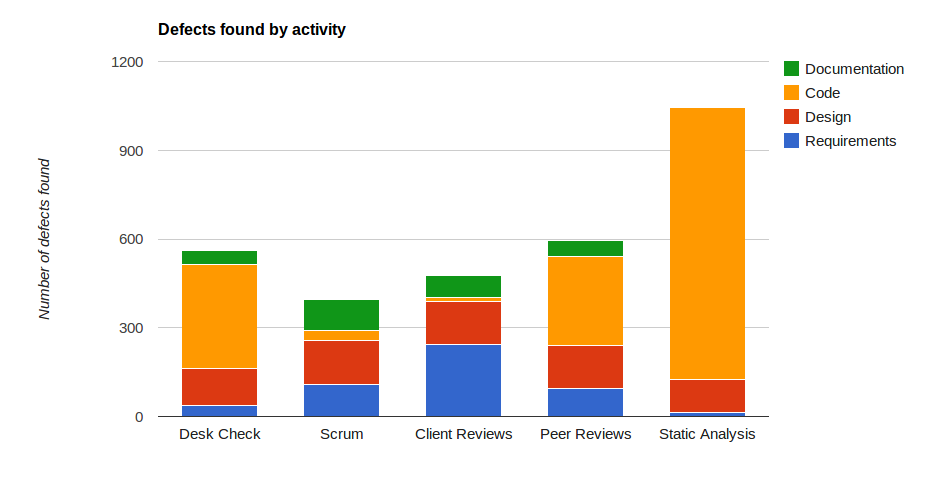
\includegraphics[width=1.0\textwidth]{image/pretest-efficiency.png}
\end{center}
\caption{Efficiency of pretest defect prevention}
\label{fig:pretest-efficiency}
\end{figure}


\textbf{Testing.} Using traditional testing methods in startup environment is a topic which has to be planned per project. As LSD divides testing in developer and customer tests, each project has to decide which of the traditional methods of testing have the best result when applied. Plain unit testing and subroutine testing can be relevant in some situations, but the use of excessive unit testing in pursuit for full test coverage can be waste of time and resources. In startup environment, the development is usually done as a cross-application development covering full features. In this kind of development the testing should be focused on testing the application as a whole. Though, testing parts of the application can be useful and even necessary depending on the software.

% \section{The Don'ts - Things To Avoid}

% DEFECT TRACKING IS A WASTE
% Liittyy vahvasti Leanin Wasteen
% Älä raportoi bugeja, joista tiedät, ettei niitä korjata
% Ei turhia raportteja
% ECO: Cost per defect => paras tulos bugisimmassa projektissa
% ECO:  p. 127 harmful combinations PREVENTIVE

% Right the first time LSD p.19(?)

% Capers Jones has interpreted from the research of multiple years of software quality that there can be harmful combinations of methods used. Even when combinind harmful methods with helpful ones, the harmful method seem to end up winning. That is, defect potentials are raising instead of coming down. Some methods combined with others can raise the defect potentials and make applications risky with a change of failure.
